\documentclass[10pt]{book}
\usepackage[text=17cm,left=2.5cm,right=2.5cm, headsep=20pt, top=2.5cm, bottom = 2cm,letterpaper,showframe = false]{geometry} %configuración página
\usepackage{latexsym,amsmath,amssymb,amsfonts} %(símbolos de la AMS).7
\parindent = 0cm  %sangria
\usepackage[T1]{fontenc} %acentos en español
\usepackage[spanish]{babel} %español capitulos y secciones
\usepackage{graphicx} %gráficos y figuras.

%---------------FORMATO de letra--------------------%

\usepackage{lmodern} % tipos de letras
\usepackage{titlesec} %formato de títulos
\usepackage[backref=page]{hyperref} %hipervinculos
\usepackage{multicol} %columnas
\usepackage{tcolorbox, empheq} %cajas
\usepackage{enumerate} %indice enumerado
\usepackage{marginnote}%notas en el margen
\tcbuselibrary{skins,breakable,listings,theorems}
\usepackage[Bjornstrup]{fncychap}%diseño de portada de capitulos
\usepackage[all]{xy}%flechas
\counterwithout{footnote}{chapter}
\usepackage{xcolor}
\usepackage[htt]{hyphenat}
%--------------------GRÀFICOS--------------------------

\usepackage{tkz-fct}

%---------------------------------

\titleformat*{\section}{\LARGE\bfseries\rmfamily}
\titleformat*{\subsection}{\Large\bfseries\rmfamily}
\titleformat*{\subsubsection}{\large\bfseries\rmfamily}
\titleformat*{\paragraph}{\normalsize\bfseries\rmfamily}
\titleformat*{\subparagraph}{\small\bfseries\rmfamily}

%------------------------------------------

\renewcommand{\labelenumi}{\Roman{enumi}.}%primer piso II) enumerate
\renewcommand{\labelenumii}{\arabic{enumii}$)$}%segundo piso 2)
\renewcommand{\labelenumiii}{\alph{enumiii}$)$}%tercer piso a)
\renewcommand{\labelenumiv}{$\bullet$}%cuarto piso (punto)

%----------Formato título de capítulos-------------

\usepackage{titlesec}
\renewcommand{\thechapter}{\arabic{chapter}}
\titleformat{\chapter}[display]
{\titlerule[2pt]
\vspace{4ex}\bfseries\sffamily\huge}
{\filleft\Huge\thechapter}
{2ex}
{\filleft}

\begin{document}

\normalfont
\input xy
\xyoption{all}
\author{\Large Apuntes por FODE}
\title{\small Landreth / Colander \\ \vspace{1cm} \large HISTORIA DEL PENSAMIENTO ECONÓMICO}
\date{}
\pagestyle{empty}
\maketitle
\thispagestyle{empty}
\let\cleardoublepage\clearpage
\tableofcontents								%indice


%------------------------------------------
 
\let\cleardoublepage\clearpage

\chapter{Introducción}
\section*{El principal tema de interés del pensamientoe económico moderno}
A principios de la década de 1900 algunas sociedades adoptaron un sistema de planificación central, que implicaba el control estatal de la asignación de los recursos. En Europa oriental, se observan movimientos para pasar de una economía autoritaria a una economía de mercado, cuyos resultados son inciertos.\\
Las sociedades modernas de mercado utilizan \textbf{la fuerza, la tradición y la autoridad, además de los mercados.}\\
\subsection*{Divisiones de la teoría económica moderna}
En el pensamiento económico moderno, los problemas relacionados con la escasez relativa generalmente se dividen en microeconomía y macroeconomía. La microeconomía analiza las cuestiones de la asignación y la distribución. . La macroeconomía analiza las cuestiones de la estabilidad y el crecimiento. 
\section*{Nuestro enfoque de la historia del pensamiento económico}
\subsection*{Enfoque relativista y absolutista}
A los historiadores relativistas les interesan las fuerzas históricas, económicas, sociológicas y políticas que llevaron a los hombres y a las mujeres a examinar ciertas cuestiones económicas y  el modo en que estas fuerzas determinaron el contenido de la teoría emergente. Sostienen que la historia desempeña un papel importante en el desarrollo de todas las teorías económicas. Un relativista haría hincapié, por ejemplo, en las relaciones entre la aparición y el contenido de la economía clásica y la industrialización de Inglaterra, entre la economía ricardiana y el conflicto entre los terratenientes y los capitalistas ingleses y entre la economía keynesiana y la Gran Depresión de los años 30.\\
Los historiadores absolutistas ponen el acento en las fuerzas internas, como la creciente profesionalización de la economía, para explicar el desarrollo de la teoría económica. Los absolutistas sostienen que el progreso de la teoría no refleja meramente las circunstancias históricas sino que depende del descubrimiento y la explicación de problemas o paradojas sin resolver por parte de profesionales formados que reaccionan a los avances intelectuales que surgen en el seno de la profesión. Según este enfoque, es posible ordenar las teorías en términos absolutos según su valor; lo más probable es que la teoría más reciente contenga menos errores y se aproxime más a la verdad que las teorías anteriores.\\
Es más fructífero concebir la historia del pensamiento económico como un proceso dinámico de interacción entre las fuerzas externas e internas de la disciplina que dan origen a nuevos avances teóricos.
\subsection*{Economistas ortodoxos y heterodoxos}
Una manera de comprender las cuestiones que separan a los autores ortodoxos de los heterodoxos es examinar las preguntas a las que trataban de responder. Mientras que los teóricos ortodoxos modernos se han ocupado principalmente de los cuatro problemas de la asignación, la distribución, la estabilidad y el crecimiento, los economistas heterodoxos han estudiado las fuerzas que provocan cambios en la sociedad y la economía.
\section*{El papel de los economistas heterodoxos}
\subsection*{Cómo influyen los economistas discrepantes en el pensamiento económico y en la profesión}
Una manera de comprender el papel de los economistas discrepantes es examinar un segmento de la historia del pensamiento económico. 

\subsection*{La economía como arte y como ciencia}
Tal vez la distinción más importante en el pensamiento económico sea la que se hace entre el arte de la economía, la economía positiva y la economía normativa. La economíapositiva se ocupa de las fuerzas que gobiernan la actividad económica.\\
La economía normativa se ocupa explícitamente de qué debe ser.\\
La distinción es importante porque la economía positiva y el arte de la economía tienen metodologías muy distintas. La metodología de la economía positiva es formal y abstracta; trata de separar las fuerzas económicas de las fuerzas políticas y sociales. La metodología del arte de la economía es más compleja, ya que se ocupa de la política económica y debe abordar las relaciones entre la política, las fuerzas sociales y las fuerzas económicas.\\
\subsection*{La importancia de la verificación empírica}
$“$Abductivo$”$ es el nombre que dio un filósofo pragmático, Charles Peirce, a una combinación específica del enfoque inductivo y el deductivo. El concepto abductivo es importante para la economía y otros estudios de sistemas complejos. El razonamiento abductivo utiliza tanto la deducción como la inducción para dar una explicación razonable a lo que ocurre. Conjuga la historia, las instituciones y el estudio empírico para comprenderlo; sin embargo, no pretende ofrecer una teoría definitiva, ya que, cuando se trata de un complejo sistema, no es posible llegar a tener una teoría definitiva.\\
\part{La economía preclásica} 

\chapter{Los comienzos del pensamiento económico preclásico}
Los pensadores chinos, griegos, árabe-islámicos y escolásticos no analizaron la economía como una disciplina independiente; estaban interesados en cuestiones mucho más amplias y filosóficas. Y como la actividad económica que observaron en esos primeros tiempos no estaba organizada en un sistema de mercado como el que conocemos hoy, no se ocuparon de la naturaleza y el significado de un sistema de precios sino de cuestiones éticas relacionadas con la justicia y la equidad. Sin embargo, sus ideas sobre algunos fenómenos económicos sirvieron de base a pensadores posteriores. La excepción a esta generalización es Guan Zyong, cuyas obras, aunque adelantadas a su tiempo, eran desconocidas en Occidente.\\
Los pensadores griegos, especialmente Hesiodo y Jenofonte, estudiaron la administración de los recursos en el ámbito del hogar y del productor y extrajeron sus conclusiones sobre la eficiencia y su relación con una división correcta del trabajo. Aristóteles y otros griegos examinaron el papel de la propiedad privada y de los incentivos. En su análisis de las necesidades y los deseos, Aristóteles planteó cuestiones eternas sobre el fin de la vida, cuestiones que se convirtieron en el tema de interés en los análisis posteriores de los escolásticos.\\
Durante la Edad Media, se tradujeron muchos escritos griegos al árabe y del árabe al latín. Los estudiosos árabes influyeron, pues, en el pensamiento escolástico en los campos de la filosofía, la ética, las ciencias y la economía hasta un grado que no se ha reconocido totalmente hasta los últimos cincuenta años. Y aunque la doctrina religiosa musulmana y la cristiana eran esencialmente hostiles a la actividad económica, no pudieron eliminar todas las actividades económicas. Al-Ghazali e Ibn Khaldun, al tratar de comprender su época, consiguieron, pues, aportar algunas ideas útiles sobre la actividad económica y contribuyeron así al largo proceso histórico de construcción de
los cimientos del conocimiento de la economía.

\chapter{El mercatilismo, la fisiocracia y otros precursores del pensamiento económico clásico.}
\section*{El mercatilismo}
\subsection*{Aportaciones teóricas del mercantilismo}
El logro más importante de los últimos mercantilistas posiblemente fuera el reconocimiento explícito de la posibilidad de analizar la economía. Este avance representó la transferencia a las ciencias sociales de actitudes que imperaban por entonces en las ciencias físicas. Se materializó plenamente tras el periodo en que vivió Isaac Newton (1642–1727) y sus efectos aún se sienten hoy. La sustitución del análisis moral de los escolásticos por el análisis de causa–efecto no representa, sin embargo, una clara ruptura con el pasado, ya que el análisis lógico fue utilizado por algunos escolásticos y la moralización aún existe en la literatura económica moderna. Pero la idea de que las leyes de la economía podían descubrirse por medio de los mismos métodos que revelaron las leyes de la física fue un paso importante para el desarrollo posterior de la teoría económica. Muchos mercantilistas veían una causalidad muy mecánica en la economía y creían que si se comprendían las reglas de esta causalidad, se podría controlar la economía. Por tanto, con una acertada legislación sería posible influir positivamente en el curso de los acontecimientos económicos y el análisis económico indicaría que tipos de intervención del Estado lograrían el fin perseguido. Los mercantilistas se dieron cuenta, sin embargo, de que la interferencia del Estado no debe ser caprichosa o complicar verdades económicas básicas como la ley de la oferta y la demanda. Algunos dedujeron correctamente, por ejemplo, que si se fijaban unos precios máximos inferiores a los de equilibrio, había exceso de demanda y escasez. Los mercantilistas posteriores aplicaron frecuentemente los conceptos de hombre económico y el motivo de los beneficios para estimular la actividad económica. Sostenían que los gobiernos no pueden cambiar la naturaleza básica de los seres humanos, especialmente sus impulsos egoístas. El político considera dados estos factores e intenta crear una serie de leyes e instituciones que canalicen estos impulsos para aumentar el poder y la prosperidad de la nación. Como veremos, muchos de los mercantilistas posteriores se dieron cuenta de los graves errores analíticos de sus predecesores. Reconocieron, por ejemplo, que la cantidad de dinero no es una medida de la riqueza de una nación, que todas las naciones no podían tener una balanza comercial favorable, que ningún país podía tener una balanza comercial favorable a largo plazo, que el comercio puede ser mutuamente beneficioso para las naciones y que la especialización y la división del trabajo beneficiarían a las naciones que las practicaran. Un creciente número de autores recomendó una reducción del grado de intervención del Estado. La literatura mercantilista contiene, pues, afirmaciones en las que se observa un incipiente liberalismo clásico.

\section*{Precursores influyentes del pensamiento clásico}
\subsection*{Thomas Mun}
Su pensamiento era típicamente mercantilista, en el sentido de que confundía la riqueza de una nación con sus reservas de metales preciosos y, por tanto, abogaba por una balanza comercial favorable y la entrada de oro y plata para saldarla. Creía que el gobierno debía regular el comercio exterior para conseguir una balanza favorable, fomentar la importación de materias primas baratas y la exportación de bienes manufacturados, aprobar aranceles protectores sobre los bienes manufacturados importados y adoptar otras medidas para aumentar la población y mantener los salarios en un nivel bajo y competitivo.\\
Cuando se publicó la última edición del famoso libro de Mun en 1755, muchos de los mercantilistas más perspicaces estaban dándose cuenta de los graves errores del paradigma mercantilista. Estos mercantilistas liberales estaban comenzando a formular los fundamentos intelectuales de la obra Wealth of Nations de Smith.

\subsection*{William Petty}
Es el primer autor que defendió la medición de las variables económicas. \\
\textbf{Political Arithmetic} de Petty se escribió en 1676, pero no se publicó hasta 1690. Petty parecía ser consciente de que estaba abriendo nuevos caminos al analizar la metodología de la aritmética política.\\
Petty parece que fue quien primero abogó explícitamente por el uso de lo que llamaríamos técnicas estadísticas para medir los fenómenos sociales. Trató de medir la población, la renta nacional, las exportaciones, las importaciones y el stock de capital de una nación. Sus métodos eran increíblemente rudimentarios, lo que llevó a Adam Smith a decir que la aritmética política le parecía de poca utilidad.\\

\subsection*{Bernard Mandeville}
Su obra \textbf{Fable of the Bees; Or, Private Vices, Publick Benefits (1714)} no sólo provocó a sus contemporáneos sino que ha continuado siendo de interés para los estudiosos de la literatura, la filosofía, la psicología y la economía. Keynes dedica dos páginas de la General Theory a analizar positivamente a Mandeville.\\
Los impulsos egoístas racionales de los seres humanos promovían el bien social porque el sentimiento moral atemperaba el egoísmo y permitía comprender la diferencia entre el bien y el mal y elegir el camino correcto. Mandeville sostenía que el egoísmo era un vicio moral, pero que de los actos egoístas podía surgir el bien social si estos actos eran debidamente canalizados por el gobierno.\\

\subsection*{David Hume}
Hume abrazó las ideas de John Locke, que pensaba que el nivel de actividad económica de una economía depende de la cantidad de dinero y de su velocidad, y realizó una descripción razonablemente completa de las relaciones entre la balanza comercial de un país, la cantidad de dinero y el nivel general de precios.\\
Según Hume, una economía no podía mantener continuamente una balanza comercial favorable, como defendían muchos mercantilistas. Una balanza comercial favorable provocaba un aumento de la cantidad de oro y plata (metales preciosos) dentro de la economía. El aumento de la cantidad de dinero provocaba una subida del nivel de precios en la economía que tenía la balanza comercial favorable. Si un país tenía una balanza comercial favorable, algún otro u otros tenían que tener una balanza desfavorable.\\
Los mercantilistas habían afirmado que las variaciones de la oferta monetaria podían aumentar la producción real. Los clásicos sostenían que la producción real no dependía de la cantidad de dinero sino de fuerzas reales: la oferta de trabajo, los recursos naturales, los bienes de capital y la estructura institucional.\\
\textbf{Hume buscó una conexión entre la libertad económica –la libertad para vender nuestros recursos, ya fuera trabajo o no, en el momento, en el lugar y al precio que quisiéramos; la libertad para producir y vender los frutos de nuestras actividades; y la libertad para comprar productos o factores sin limitaciones impuestas por fuerzas externas– y la libertad política. Hume sostenía que el aumento de la libertad económica y el aumento de la libertad política iban unidos.}\\
Hume fue un precursor de la distinción que hicieron más tarde Nassau Senior, John Neville Keynes y Lionel Robbins entre las afirmaciones positivas y las normativas. Que lo que debe ser (afirmaciones normativas) no puede derivarse de lo que es (afirmaciones positivas) se conoce con el nombre de Máxima de Hume.

\subsection*{Richard Cantillon}
Dados unos mercados competitivos en los que los empresarios buscan clientes en los mercados de bienes finales y compiten entre sí en los mercados de factores, Cantillon fue capaz de señalar los procesos de ajuste que se producen cuando cambian las demandas, los costes, la tecnología u otros factores.\\
Dividió la economía en sectores y analizó el flujo de renta entre ellos; aunque no formuló explícitamente una tabla económica para representar estos flujos, influyó claramente en Quesnay, quien sí lo hizo.

\section*{La fisiocracia}
s. Éstos se dieron cuenta de la relación entre los sectores de la economía y analizaron el funcionamiento de los mercados no regulados. La fisiocracia tuvo un líder intelectual reconocido, François Quesnay.

    \subsection*{Ley natural}
    Sostenían que las leyes naturales gobernaban el funcionamiento de la economía y que, aunque estas leyes eran independientes de la voluntad humana, los hombres podían descubrirlas objetivamente, como podían descubrir las leyes de las ciencias naturales. Esta idea contribuyó significativamente al desarrollo de la economía y de las ciencias sociales.\\


    \subsection*{La interdependencia de una economía}
    Lo que más interesaba a los fisiócratas era el proceso macroeconómico de desarrollo. n. Los fisiócratas no centraron la atención en el dinero sino en las fuerzas reales que conducen al desarrollo económico. En respuesta a la idea mercantilista de que era el comercio el que creaba riqueza, estudiaron la creación de valor físico y llegaron a la conclusión de que el origen de la riqueza estaba en la agricultura, es decir, en la naturaleza.\\
    En la economía de su tiempo, se producían más bienes de los que se necesitaban para pagar los costes reales que tenía para la sociedad la producción de esos bienes, por lo que se generaba un excedente económico. Su búsqueda del origen y la magnitud de este excedente los llevó a la idea del producto neto.\\
    Los agricultores se colocan en el centro del flujo circular porque (según los fisiócratas) la tierra es el único factor que genera un producto neto.

    \subsection*{La política económica fisiócrata}
    Aunque los fisiócratas no desarrollaron una teoría coherente de los precios, llegaron a la conclusión de que la libre competencia conducía al mejor precio y de que la sociedad se beneficiaba si los individuos buscaban su propio provecho.\\
    El Estado debía seguir una política de laissez faire, es decir, no intervenir. Esta idea, en manos de Adam Smith y de los economistas posteriores, tuvo enorme importancia en la formación de la ideología de la civilización occidental.

\section*{El pensamiento económico Español}
El interés por el pensamiento económico español anterior a Smith se ha acrecentado en los últimos cincuenta años debido en gran parte a los estudios de Marjorie Grice-Hutchinson, que ha escrito mucho sobre el pensamiento económico en los seiscientos años anteriores a la obra Wealth of Nations de Adam Smith.\\
Tras el descubrimiento del Nuevo Mundo en 1492 por Colón, España se convirtió en un importante agente económico en Europa como consecuencia de su énfasis en la adquisición de oro y plata por el medio que fuera, principalmente en lo que hoy es México y en América Central y del Sur. Esta entrada de oro en España pronto provocó una subida de los niveles de precios en todo el país.\\
En 1556, trece años antes que Jean Bodin, Azpilcueta demostró tener un conocimiento razonablemente profundo de lo que hoy llamamos teoría cuantitativa del dinero. Esta teoría explica que el factor clave que altera el nivel general de precios es la cantidad de dinero en circulación.\\ 
La formulación que hace Azpilcueta de este principio es notablemente buena: $"$En las tierras donde hay gran falta de dinero, todas las otras cosas vendibles, y aun las manos y trabajo de los hombres se dan por menos dinero que donde hay abundancia de él; como por la experiencia se ve que en Francia, donde hay menos dinero que en España, valen mucho menos el pan, el vino, los paños, las manos y los trabajos; y aun en España, cuando había menos dinero, por mucho menos se daban las cosas vendibles, las manos y los trabajos de los hombres, que después de que las Indias fueran descubiertas, la cubrieron de oro y plata. La causa es que el dinero vale más donde y cuando falta que donde y cuando es abundante$"$.\\
He aquí su magnífica exposición de cómo se veía en el siglo XVII lo que hoy llamaríamos leyes de la demanda y la oferta y la teoría cuantitativa del dinero: $"$ Son muchas las circunstancias que hacen fluctuar el precio de las cosas al alza o a la baja. Así, por ejemplo, la escasez de los bienes, debida a la mala cosecha o a causas semejantes, hace subir el justo precio. La abundancia, sin embargo, lo hace descender. El número de compradores que concurren al mercado, en unas épocas mayor que en otras, y su mayor deseo de comprar, lo hacen también subir. Igualmente, la mayor necesidad que muchos tienen de algún bien especial en determinado momento, supuesta la misma cantidad de dicho bien, hace que su precio aumente, como sucede con los caballos, que valen más cuando la guerra está próxima que en tiempos de paz. De igual forma, la falta de dinero en un lugar determinado hace que el precio de los demás bienes descienda, y la abundancia de dinero hace que el precio suba. Cuanto menor es la cantidad de dinero en un sitio, más aumenta su valor y, por tanto, caeteris paribus, con la misma cantidad de dinero se pueden comprar más cosas$"$.

\section{Resumen}
Los mercantilistas y los fisiócratas hicieron útiles aportaciones a la teoría económica, de las cuales la más importante fue su reconocimiento de que la economía podía estudiarse formalmente. Al mismo tiempo, estos autores desarrollaron una técnica abstracta para descubrirlas leyes que regulaban la economía. Fueron los primeros en construir modelos en economía; como la teoría económica se basa en el proceso abstracto de construcción de modelos, es razonable considerar que los mercantilistas y los fisiócratas fueron los primeros que desarrollaron una teoría económica.\\
Los mercantilistas lograron formularlas primeras ideas tentativas sobre el papel del dinero en la determinación del nivel general de precios y sobre los efectos que producía la balanza comercial exterior en la actividad económica interior. La aportación más significativa de los fisiócratas fue su concepto de la interdependencia de los distintos sectores de una economía.\\
Los mercantilistas y los escolásticos pensaban que existía un conflicto fundamental en la economía y concebían el comercio como un proceso en el que una de las partes sale ganando a expensas de otra. Ambos abogaron, pues, por la intervención del gobierno o de la Iglesia en la economía. Los fisiócratas pensaban, por el contrario, que la resolución de los conflictos inherentes a la escasez relativa era esencialmente armoniosa. No recomendaron la intervención en la economía sino el laissez faire y, por tanto, influyeron notablemente en Adam Smith y en el desarrollo posterior de la política económica. Algunos autores ingleses de este periodo no encajan perfectamente ni en el mercantilismo ni en el pensamiento clásico. Fueron ellos los que rechazaron las ideas mercantilistas más burdas del conflicto inherente al comercio, quienes rechazaron la necesidad de mantener siempre una balanza comercial favorable y quienes se dieron cuenta de cómo funcionan los mercados para coordinar las actividades económicas individuales. Estos mercantilistas liberales y los fisiócratas dieron a Adam Smith las herramientas con las que levantar el edificio de la economía política.\\
Algunos estudios recientes han revelado la existencia de un grupo bastante sólido de aportaciones españolas a nuestra comprensión de la economía. Entre la década de 1500 y finales de la década de 1700, el conocimiento español del funcionamiento de la economía aumentó tanto que al final del periodo algunos autores españoles rivalizaron con los últimos mercantilistas y primeros clásicos liberales ingleses en su comprensión del papel que desempeñan los mercados en el desarrollo económico.\\ 
Aunque hemos expuesto a grandes rasgos las ideas de los mercantilistas y los fisiócratas, también hemos estudiado autores concretos. William Petty, que fue esencialmente un mercantilista, fue importante porque representa el primer intento de basar la economía en la observación empírica. El rechazo de Smith de la aritmética política y los problemas para conseguir datos razonablemente exactos retrasaron casi cien años el avance hacia la cuantificación. Cantillon fue un creativo pensador analítico que hizo importantes progresos en el conocimiento del funcionamiento de un sistema de mercado y que siguió el deseo de Petty de cuantificar el razonamiento económico. Desgraciadamente, apenas influyó en el desarrollo posterior del pensamiento económico. Mandeville, mercantilista, fue un buen representante del subconsumismo y un mordaz crítico de los moralistas sentimentales (Shaftesbury, Hutcheson, Smith).\\
David Hume, que mantenía una estrecha amistad con Adam Smith, fue el otro destacado intelectual de la segunda mitad del siglo XVIII; su interés esporádico por el campo de la economía lo llevó a hacer importantes aportaciones al pensamiento económico. Aunque Hume nunca fue capaz de liberarse por completo de las ideas del mercantilismo, sí refutó un buen número de burdas ideas mercantilistas sobre el mantenimiento de una balanza comercial favorable. Su análisis mostró que una balanza comercial dada provocaba variaciones en los precios, las exportaciones y las importaciones que invertían finalmente esa balanza comercial. Probablemente nada sintetice mejor la desaparición del mercantilismo como una idea aceptable, pero no como un conjunto de medidas utilizadas para sacar ventaja, que la siguiente declaración de David Hume: “Me atrevo, pues, a reconocer, que no sólo como hombre sino como súbdito británico, hago votos por el florecimiento del comercio de Alemania, de España, de Italia e incluso de la propia Francia.\\
Antes de que Smith publicara su famosa obra, algunos autores habían logrado hacer importantes avances en el conocimiento del funcionamiento de un sistema económico y las erróneas medidas de los mercantilistas y los fisiócratas. Pero nadie había sido capaz de reunirlo todo de una forma que llamara la atención de sus contemporáneos. Éste iba a ser el papel de Adam Smith, de quien nos ocuparemos en el primer capítulo de la Segunda parte. Se convirtió en el padre de la economía política y en la primera gran figura de la lista de economistas ortodoxos.

\part{El pensamiento económico clásico y sus críticos}
\textbf{Los tres grandes Los tres grandes tratados del periodo clásico son Inquiry into the Nature and Causes of the Wealth of Nations (1776) de Adam Smith (1723–1790), On the Principles of Political Economy and Taxation (1817) de David Ricardo (1772–1823) y Principles of Political Economy (1848) de John Stuart Mill (1806–1873).} Otros dos pensadores fundamentales, Malthus y Marx, aunque son clásicos en algunos aspectos, son más importantes como críticos de la economía clásica que como defensores de ella. La teoría de la población de Thomas Malthus (1766–1834) coincide con la teoría clásica, pero Malthus se alejó significativamente de la tradición clásica ortodoxa en su análisis de algunos aspectos macroeconómicos de la economía y en su defensa del papel y la importancia de la clase terrateniente. \\
El pensamiento marxista constituye el ejemplo más significativo de pensamiento económico que considera que el sistema económico está lleno de conflictos que las fuerzas del mercado no pueden resolver.\\
La segunda característica de la escuela clásica es su preocupación por el crecimiento económico. Los economistas clásicos, como eran esencialmente de orientación macroeconómica –si bien en un sentido muy distinto al de los macroeconomistas modernos– trataron de descubrir las fuerzas que determinan la tasa de crecimiento económico. Al igual que los que estudian las economías actuales menos desarrolladas, \textbf{los clásicos tenían un marco de referencia mucho más amplio que los macroeconomistas modernos. Se interesaron no sólo por las fuerzas económicas que determinaban el crecimiento sino también por los factores culturales, políticos, sociológicos e históricos.} Como la macroeconomía moderna ha vuelto a ocuparse de estas mismas cuestiones y supuestos al alejarse de la macroeconomía keynesiana, los macroeconomistas modernos a veces se denominan $"$nuevos economistas clásicos$"$.\\

\begin{center}
    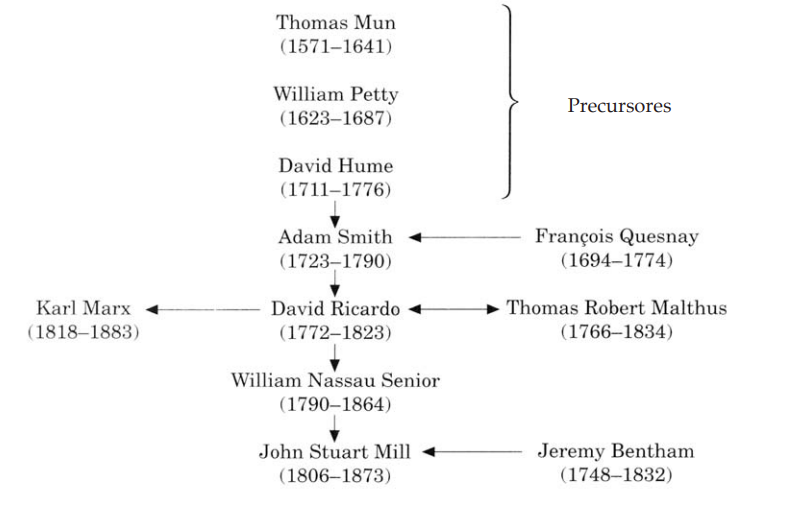
\includegraphics[width=0.8\textwidth]{imagen/influencia.png}
\end{center}

Marx señaló el conflicto económico entre los capitalistas y los trabajadores. Adaptó la teoría del valor-trabajo de los clásicos para defender su tesis de que el trabajo era explotado por los capitalistas.\\
Adam Smith se había interesado principalmente por el crecimiento económico y David Ricardo por los cambios que experimentaría a largo plazo la distribución de la renta en el capitalismo. El análisis económico de Marx forma parte de un interés más general por las fuerzas que provocan el cambio histórico, pero algunas de estas mismas cuestiones dinámicas de las que se ocuparon los clásicos también interesaron a Marx: ¿qué ocurrirá con la distribución de la renta con el paso del tiempo? ¿Cómo evolucionará la tasa de beneficios? ¿Cuáles son las perspectivas del nivel de bienestar de las masas?\\
\textbf{. Para los clásicos, los agentes importantes eran los capitalistas, los terratenientes y los trabajadores. La teoría clásica es en cierto sentido un análisis de las funciones económicas y del futuro de estas clases.\\
. Para los clásicos, el motivo del beneficio de los capitalistas conducía a una asignación eficiente del capital en la economía y al ahorro, lo cual fomentaba el crecimiento y la riqueza. Para Marx, las actividades de los capitalistas perjudicaban en última instancia al proletariado y a la sociedad. La economía clásica es una oda al capitalismo; la de Marx es una oda sobre sus fallos.}

\chapter{Adam Smith}
\section*{Las variedades de intereses de Adam Smith}
Observó, por ejemplo, la existencia de importantes conexiones entre la libertad económica y la libertad política, entre los derechos de propiedad privada y un Estado justo y entre los individuos que actúan movidos, en parte, por el interés personal y, en parte, por la preocupación por las consecuencias de sus actos para los demás.\\
Smith recibió la influencia de su maestro, Francis Hutcheson (1694–1746) y de David Hume (1711–1776).\\
\textbf{ Se considera que las ideas religiosas que ponen el acento en las virtudes del trabajo y el ahorro han contribuido significativamente a fomentar la aparición de la sociedad económica moderna.}\\
\textbf{Creían que de la misma manera que Newton había encontrado orden y armonía en el mundo físico por medio de un riguroso análisis, podrían descubrir las leyes naturales que gobiernan la sociedad.}.\\
Los economistas modernos dirían de Smith que era un teórico macroeconómico interesado por las fuerzas que determinan el crecimiento económico.

\section*{El análisis de los mercados de Smith y sus conclusiones sobre la política económica}
\textbf{e la importancia de Smith en la historia del pensamiento económico se debe (1) a su profunda comprensión de la interdependencia de la economía y (2) a su influencia en la política económica.}

\subsection*{Política económica contextual}
La defensa del laissez faire de Smith tiene sus orígenes en un enfoque metodológico que se pregunta si la experiencia demuestra que la intervención del Estado produce mejores resultados que el funcionamiento incontrolado de los mercados? Smith reconocía que los mercados a menudo no generan resultados sociales ideales, pero la realidad de su época lo convenció de que los resultados de la intervención del Estado eran menos aceptables que los que producía el libre mercado. Smith defendía, pues, el laissez faire, pero no porque creyera que los mercados eran perfectos sino porque teniendo en cuenta la historia y la estructura institucional de la Inglaterra de su época, los mercados normalmente producían mejores resultados que la intervención del Estado.\\

\subsection*{El orden natural, la armonía y el laissez faire}
El silogismo del que extrajo Smith su principal conclusión sobre la política económica es muy sencillo. Los seres humanos son racionales y calculadores y actúan movidos por el interés personal. . Si no se interfiere en sus comportamientos, buscan su propio interés y al promoverlo, promueven el interés de la sociedad. El gobierno no debe interferir en este proceso, por lo que debe seguir una política de laissez faire.\\
. Smith muestra que los capitalistas no actúan movidos por motivos altruistas sino por el deseo de obtener beneficios.\\
Smith llegó a la conclusión de que es maravilloso que el mercado, sin planificación o dirección gubernamental alguna, satisfaga los deseos de los consumidores con el menor coste social posible. \textbf{En la terminología de la economía moderna, llegó a la conclusión de que los mercados competitivos asignan óptimamente los recursos sin intervención del Estado.}

\subsection*{El funcionamiento de los mercados competitivos}
En condiciones de competencia en los mercados y en ausencia de intervención del Estado, los precios naturales (precios a largo plazo) resultantes generan una asignación óptima de los recursos, en el sentido de que los consumidores reciben los bienes que desean con el menor coste posible y se garantizan las máximas tasas de crecimiento.\\
Reconoció el deseo de los hombres de negocios de monopolizar el comercio aunando fuerzas y aunque no fue capaz de especificar cuál sería el precio monopolístico, reconoció que los monopolistas extraen un precio más alto limitando la producción. \\
Los argumentos de Smith en contra de la intervención del Estado en la economía tenían bases políticas, filosóficas y económicas. Sostenía que, en general, la interferencia del Estado no era deseable, ya que violaba los derechos y las libertades naturales de los individuos.\\ 
\textbf{. Smith creía que muchos de los argumentos mercantilistas a favor de la intervención del Estado, aunque pretendían promover el bien social, en realidad eran interesados. Si los gobiernos fueran diferentes, podrían promover el bien social, pero dado como son, inevitablemente hacen más daño que bien.}

\subsection*{El capital y los capitalistas}
\textbf{La riqueza de un país depende de la acumulación de capital, ya que ésta es la que determina la división del trabajo y la proporción de la población dedicada al trabajo productivo. En segundo lugar, Smith llegó a la conclusión de que la acumulación de capital también lleva al desarrollo económico. En tercer lugar, el interés privado, junto con la acumulación de capital, conduce a una asignación óptima del capital a los distintos sectores.\\
La fuente del capital en una economía basada en la propiedad privada es el ahorro de los individuos. Smith creía que el trabajo no podía acumular capital porque el nivel de salarios sólo permitía satisfacer los deseos inmediatos de consumo. Los miembros de la clase terrateniente tienen suficiente renta para acumular capital, pero la gastan en trabajo improductivo para satisfacer su inmensos deseos de gozar de un elevado nivel de vida.}\\

\subsection*{La influencia de Smith en la política económica}
Su principal conclusión sobre la política económica fue que el gobierno debía seguir una política de laissez faire. La influencia de esta conclusión en la política económica del mundo industrializado, especialmente de Estados Unidos, ha sido inmensa. Se ha convertido en la ideología económica de su sociedad y se intenta promover en las zonas subdesarrolladas del mundo. Es posible que ninguna idea y ningún escritor hayan tenido más influencia en el desarrollo de nuestra economía y nuestra sociedad.

\section*{La naturaleza y las causas de la riqueza de las naciones}
Para Smith, la riqueza era un flujo anual de bienes y servicios, no un fondo acumulado de metales preciosos. También demostró comprender la relación entre las exportaciones y las importaciones y darse cuenta de que el papel fundamental de las exportaciones era financiar las importaciones.\\
\textbf{Smith sugirió, además, que la riqueza de las naciones se midiera en unidades per cápita.} Hoy cuando se dice, por ejemplo, que Inglaterra es un país más rico que China, se entiende que la comparación no se basa en la producción o en la renta total de los dos países sino en la renta per cápita de la población.\\

\subsection*{Causas de la riqueza de las naciones}
Smith sostenía que la riqueza de una nación, lo que hoy llamamos la renta de un país, depende (1) de la productividad del trabajo y (2) de la proporción de trabajadores que tienen un empleo útil o productivo. Como suponía que la economía lograba utilizar automáticamente a pleno rendimiento sus recursos, sólo examinó las fuerzas que determinan la capacidad de una nación para producir bienes y servicios.

\subsubsection*{La productividad del trabajo} 
La productividad del trabajo depende de la división del trabajo. La división del trabajo depende, a su vez, de lo que Smith llamó extensión del mercado y de la acumulación de capital. Cuanto mayor es el mercado, mayor es el volumen que puede vender y mayores las oportunidades de introducir la división del trabajo.\\
\textbf{Una importante función del capitalista es poner los medios necesarios para cubrir el hueco entre el momento en el que comienza la producción y el momento en el que se vende el producto final}.\\

\subsubsection*{Trabajo productivo e improductivo}
Como defensor del cambio del orden social y económico, presupone que las actividades de los capitalistas, que aumentan la producción de bienes reales, son beneficiosas para el crecimiento y el desarrollo económicos, mientras que los gastos de los terratenientes en sirvientes y bienes intangibles son despilfarradores. Un hombre se hace rico contratando una multitud de trabajadores; se hace pobre manteniendo una multitud de sirvientes.\\
Como el gasto público en trabajo improductivo impide el crecimiento económico, es mejor que el Estado sea más pequeño y, por consiguiente, que los impuestos que pagan los capitalistas sean más bajos para que puedan acumular más capital.

\subsection*{Resumen de las causas de la riqueza de las naciones}
El valor del producto anual de la tierra y el trabajo de una nación no puede incrementarse mediante ningún otro medio que no sea aumentando el número de trabajadores productivos o la capacidad productiva de los trabajadores que ya estaban empleados. Es evidente que el número de trabajadores productivos nunca puede incrementarse mucho si no es como consecuencia de un aumento del capital o de los fondos destinados a mantenerlos. No es posible incrementar la capacidad productiva del mismo número de trabajadores si no es como consecuencia de un aumento y de una mejora de las máquinas y los instrumentos que facilitan y abrevian el trabajo; o de una división y distribución mejores del empleo. En cualquiera de los dos casos, casi siempre es necesario más capital.\\\\

LA RIQUEZA DE LAS NACIONES depende de

\begin{enumerate}[\bfseries 1.]
    \item \textbf{Productividad del trabajo.} Que depende de la división del trabajo., y este depende de 
	\begin{enumerate}[\bfseries a.]
	    \item Extensión del mercado. Que depende de la acumulación de capital.
	    \item Acumulación de capital.
	\end{enumerate}
    \item \textbf{Cociente entre el trabajo productivo y el improductivo.} Que depende de la acumulación de capital.
\end{enumerate}

\subsection*{El comercio internacional}
En el lenguaje de la economía moderna, el trabajo tiene rendimientos crecientes (costes decrecientes) conforme va especializándose. Parte del argumento de Smith a favor de las ventajas del comercio exterior se basa en líneas generales en este concepto dinámico de rendimientos decrecientes. Smith se dio cuenta de que si dos personas tienen el mismo talento al nacer y éste no varía, ninguno de las dos obtiene ventajas si se especializan y comercian sus bienes (la nacionalidad de los individuos no influye en estos argumentos, es decir, el hecho de que uno de ellos sea inglés y el otro francés).\\
Sin embargo, si dos personas se vuelven más competentes gracias a la especialización del trabajo, los costes de producir sus productos disminuyen y las dos se benefician especializándose y comerciando. De esta idea se deriva el reconocimiento de Smith, fundamental para el desarrollo del libre comercio, de que con el tiempo cualquier país puede lograr dinámicamente ventajas absolutas de costes en la producción de ciertos bienes por medio de la especialización y de la división del trabajo y que todas las naciones pueden beneficiarse del comercio internacional resultante.\\
si se sostiene que la cantidad total de recursos de nuestro planeta es fija, el proceso de intercambio entre dos individuos o naciones requiere necesariamente que uno pierda y el otro gane. En el lenguaje de algunos economistas modernos, un intercambio económico es un “juego de suma cero”, en el que uno gana y otro pierde.\\

\section*{La teoría del valor}
Precio relativo o cuestión de valor.
\subsection*{Precios relativos}
Creía que los precios de mercado o a corto plazo son determinados tanto por la
oferta como por la demanda. Los precios naturales o de equilibrio a largo plazo generalmente dependen de los costes de producción.\\
El análisis que hace Smith de la formación de los precios relativos en la economía de su tiempo distingue dos periodos: el corto plazo y el largo plazo, y dos grandes sectores de la economía, la agricultura y el sector manufacturero. Durante el periodo a corto plazo o de mercado, Smith observó curvas de demanda de pendiente negativa y curvas de oferta de pendiente positiva tanto en el sector manufacturero como en la agricultura; por tanto, los precios de mercado dependen de la demanda y la oferta.\\
No obstante, cualquiera que sea la forma de la curva de oferta a largo plazo del sector manufacturero, en la determinación de los precios naturales se pone el énfasis principalmente en el coste de producción, énfasis que es característico de Smith y de los economistas clásicos posteriores.\\

\subsection*{El significado del valor}
\textbf{tiene dos significados distintos y unas veces expresa la utilidad de un objeto y otras el poder de compra de otros bienes que confiere la propiedad de ese objeto. Uno puede denominarse valor de uso; el otro, valor de cambio. Las cosas que tienen el máximo valor de uso a menudo tienen un escaso o nulo valor de cambio; y las que tienen el máximo valor de cambio a menudo tienen, por el contrario, un escaso o nulo valor de uso. Nada es más útil que el agua, pero con ella no se puede comprar casi nada; no se puede obtener casi nada a cambio. Un diamante, por el contrario, apenas tiene valor de uso, pero a menudo se puede cambiar por él una gran cantidad de bienes.}\\
El valor de cambio es el poder de una mercancía para comprar otros bienes, es decir, su precio. Por otra parte, el valor de uso es el poder de una mercancía para satisfacer deseos, la utilidad que se obtiene por poseer o consumir un bien.\\
Como la utilidad marginal de una mercancía a menudo disminuye cuanto mayor es la cantidad que se consume de ella, es muy posible que otra unidad de agua generara menos utilidad marginal que otra de diamantes.\\

\subsection*{Smith y los precios relativos}
Desarrollo tres teorías distintas sobre los precios relativos.\\
\begin{enumerate}[\bfseries (1)]
    \item Una teoría del valor basada en el coste del trabajo.
    \item Una teoría del valor basada en el coste de producción.
    \item Una teoría del valor basada en la cantidad de trabajo que se puede comprar.
\end{enumerate}

\subsubsection*{Teoría del valor basada en el coste del trabajo en una sociedad primitiva}
Smith reconoció que la cantidad de trabajo necesaria para producir un bien no puede medirse simplemente en horas de reloj, ya que también hay que tener en cuenta, además del tiempo   el ingenio o la cualificación y las dificultades o los aspectos desagradables de la tarea. \\
Smith trató de resolver este problema de reducir el tiempo, la dificultad y el ingenio a un denominador común manteniendo que las diferencias de tiempo, dificultad e ingenio se reflejan en los salarios que se pagan al trabajo.

\paragraph*{La cantidad de trabajo que se puede comprar en una sociedad primitiva}
Smith llegó a la conclusión de que si se necesitan dos horas para cazar un castor o dos ciervos, dos ciervos serán iguales a un castor en el mercado, es decir, el precio de un castor será el doble del precio del ciervo.

\paragraph*{Teoría del trabajo en una economía avanzada}
El modelo de Smith para una sociedad avanzada se diferencia de su modelo para una economía primitiva en dos importantes aspectos: se ha acumulado capital y ha habido apropiación de la tierra. . Los precios finales generan unos ingresos formados por los pagos de salarios, beneficios y rentas a los factores.

\subsubsection*{La teoría del valor basada en el coste de producción}
Una vez que se ha acumulado capital y ha habido apropiación de la tierra y una vez que deben pagarse beneficios y rentas, además de salarios, parece que la única explicación correcta de los precios que encontró fue una teoría basada en el coste de producción. \textbf{En una teoría basada en el coste, el valor de una mercancía depende de los pagos a todos los factores de producción: la tierra y el capital, además del trabajo}.\\
Smith sostenía que cuando hay competencia, los intereses personales del hombre de negocios, del trabajador y del terrateniente dan como resultado unos precios naturales que son iguales al coste de producción.

\section{La teoría de la distribución}
\textbf{El trabajo es el único factor de producción que posee la mayoría de los hogares; por tanto, la renta de un hogar generalmente depende del salario y del número de horas trabajadas.}\\

\subsection*{Los salarios}
Smith señaló que el trabajo se encuentra en una situación de desventaja en el proceso de negociación de los salarios.

\subsubsection*{La doctrina del fondo de salarios}
Esta
doctrina supone que hay un fondo fijo de capital destinado a pagar los salarios.

\subsection*{Los beneficios}
Los beneficios constan, pues, de dos partes: un rendimiento puro en intereses y un rendimiento por el riesgo. 

\subsection*{Las rentas}
Smith propuso cuatro teorías como mínimo de las rentas, todas ellas mutuamente contradictorias. Se dice que los orígenes de las rentas son:
\begin{enumerate}[\bfseries (1)]
    \item Las demandas del terrateniente.
    \item El monopolio.
    \item Las ventajas diferenciales.
    \item Un regalo de la naturaleza.
\end{enumerate}

Considera que la renta es determinada por el precio.

\subsection*{La evolución de la tasa de beneficios}
Predijo que la tasa de beneficios disminuiría con el paso del tiempo por tres razones:
\begin{enumerate}[\bfseries (1)]
    \item La competencia existente en el mercado de trabajo. Es decir, la subida de los salarios provocaría un descenso de los beneficios.
    \item La competencia existente en el mercado de mercancías. Es decir, que cuando se aumenta la competencia entre los productores los precios bajan y los beneficios disminuyen.
    \item La competencia en el mercado de inversión. 
\end{enumerate}

\section*{El bienestar y el nivel general de precios}

\subsection*{Capítulo 5, Libro I}
Si el bienestar se mide en función del consumo total o de la producción de la sociedad, el problema inicial que hay que resolver en el caso de una economía que produce más de un bien es encontrar la manera de sumar la producción o el consumo de los productos, por ejemplo, castores y ciervos. Una solución posible es convertir todas las mercancías a una única medida. Si $1Ca = 1Ci$, entonces un aumento de la producción de dos castores unida a una disminución de la producción de dos ciervos representa un aumento del bienestar. Puede decirse que el nuevo nivel de producción supone una mejora igual a un castor o dos ciervos. Sin embargo, si varían los precios relativos los castores y de los ciervos cuando varía su producción, es mucho más complicado medir el bienestar. En una economía en la que hay muchos productos, los precios relativos de las mercancías se expresan en una medida común, normalmente la unidad monetaria del país. En teoría y a veces en la práctica, esta medida común (en la jerga de la economía, el numerario) podría ser cualquiera de las mercancías de la economía, por ejemplo, vacas, trigo u oro. En nuestra economía, medimos la producción sumando el valor monetario de cada mercancía para obtener una suma que llamamos producto interior bruto. La única medida o nu,erario que no variaba y que pudo encontrar para evaluar los cambios del bienestar fue la desutilidad del trabajo, ya que puede decirse que una misma cantidad de trabajo tiene en todas las épocas y lugares el mismo valor para el trabajador.\\
Primero medimos las variaciones de la producción total por medio de la unidad monetaria; a continuación ajustamos la medida para tener en cuenta las variaciones del nivel general de precios de acuerdo con las variaciones del precio del oro, la plata o el trigo. Mediante este proceso, hemos convertido la renta monetaria y el precio nominal en renta real y precio real. Para medir los cambios del bienestar, comparamos a continuación la cantidad de desutilidad del trabajo que implica la producción de los diferentes productos.\\
\textbf{El bienestar aumenta si disminuye la desutilidad de la producción de este producto. Traducido al lenguaje diario, si pudiéramos producir la misma cantidad con menos trabajo, tendríamos más ocio y disfrutaríamos de más bienestar.}

\chapter{Ricardo y Marthus}

\section*{La doctrina Mathusiana sobre la población}
La tesis principal de Malthus, a saber, que la población tiende a aumentar más deprisa que las existencias de alimentos, no es suya: puede encontrarse en los escritos de otros autores, entre los que figuran Adam Smith y Bejamin Franklin. Fue, sin embargo, la presentación del problema demográfico de Malthus la que influyó significativamente en el pensamiento económico de la época y en el posterior.

\subsection*{La teoría sobre la población como una respuesta intelectual a los problemas de la época}
\subsubsection*{La tesis sobre la población}
El principio básico de Malthus, establecido en la primera edición de su ensayo, se basaba en dos supuestos:
\begin{enumerate}[\bfseries (1)]
    \item que los alimentos son necesarios para la existencia de la
humanidad y
    \item que la pasión entre los sexos es necesaria y no cambiará. 
\end{enumerate}
\textbf{Malthus llegó a la conclusión de que la población tiende a crecer a un ritmo más rápido que las existencias de alimentos.} Malthus sostenía que los seres humanos, en ausencia de mecanismos que frenen la población, tenderán a aumentar en progresión geométrica (1, 2, 4, 8, 16, ...), pero que las existencias de alimentos sólo pueden aumentar en progresión aritmética (1, 2, 3, 4, 5, ...). Afirmó que eso es la causa de la pobreza y el sufrimiento.\\ 
Llegó a la conclusión de que se desarrollarán frenos que harán que la tasa de crecimiento de la población sea acorde con la tasa de crecimiento de las existencias de alimentos. Examinó varios frenos, que varían de la primera edición a las posteriores. En la primera, postuló dos tipos de frenos, los positivos y los preventivos. Los positivos son los aumentos de la tasa de mortalidad como consecuencia de las guerras, el hambre, las enfermedades y catástrofes parecidas. Un freno preventivo es la disminución de la tasa de natalidad, que se logra posponiendo el matrimonio. En la primera edición de su ensayo sobre la población, Malthus llegó a la conclusión de que la posposición del matrimonio sólo engendraría vicio, sufrimiento y degradación del carácter, ya que habría relaciones sexuales prematrimoniales.\\

\subsubsection*{Contraversia sobre la tesis de la población}
La tesis de Malthus sobre la población tiene algunos errores evidentes. Al igual que la mayoría de sus contemporáneos, nunca analizó seriamente la posibilidad de controlar la población por medio de la contracepción, si bien muchos de los llamados neomalthusianos de épocas más recientes han abogado porlas medidas contraceptivas. Malthus confudió, además, el deseo instintivo de mantener relaciones sexuales con el deseo de tener hijos. Aunque el impulso sexual es fuerte en todas las sociedades, el aumento del nivel de prosperidad y de educación tiende a introducir una distinción entre los deseos sexuales y la decisión de tener hijos. Otra dificultad es el supuesto arbitrario de Malthus de que las reservas de alimentos no pueden aumentar más deprisa que la población. En otras palabras, no consideró la posibilidad de que el desarrollo de la tecnología agrícola permitiera aumentar lo suficiente las existencias de alimentos para alimentar a una población mayor. Pero no es justo criticar excesivamente a Malthus por esta omisión, pues los economistas nunca han desarrollado una teoría que explique la tasa de desarrollo tecnológico, por lo que históricamente han subestimado la influencia de la tecnología en la economía.\\
La tesis de Malthus sobre la población se aplicó en la teoría y la política económicas clásicas. La doctrina del fondo de salarios, desarrollada por Smith y ampliada por Ricardo y sus seguidores, implicaba que una subida del salario real del trabajo provocaría un aumento de la población, lo cual acabaría bajando el salario y devolviéndolo a su nivel anterior. Se sostenía, pues, que cualquier intento de mejorar el bienestar económico de los grupos de renta más baja de la sociedad fracasaría debido a que el volumen de población aumentaría. Por tanto, aunque los sentimientos humanitarios pidieran medidas sociales para elevar la renta de los trabajadores pobres, la lógica económica sólida decía que esos esfuerzos serían vanos.

\section*{Ricardo: Método, política económica, ámbito}

\subsection*{El método de Ricardo}
Aunque el método de Ricardo dé al observador superficial la impresión de que era un economista puramente teórico y poco práctico, la economía ricardiana está orientada en gran medida hacia la política económica. La cuestión candente en su época eran los aranceles sobre las importaciones inglesas de cereales y sus consecuencias para la distribución de la renta y Ricardo era muy consciente de esta cuestión. No obstante, sostenía taxativamente que la teoría era una condición previa para poderrealizar un análisis concreto de las cuestiones de política del mundo real.

\subsection*{Ricardo y  la economía política}
La manera de formular una buena política, utilizando a Ricardo de modelo, es dejar de lado todo lo que no es esencial y construir un modelo sumamente teórico que revele las relaciones causales entre las variables. Para conseguir extraer sólidas conclusiones teóricas puede ser necesario dejar de lado –o congelar– variables que influirían significativamente en los resultados cuando se utiliza el modelo teórico para formular la política económica.\\
Actualmente subsisten dos componentes del ricardismo: la teoría sumamente abstracta, que elimina por hipótesis tantas variables que la conclusión final es indiscutible, y la formulación no contextual de la política económica basada en modelos abstractos.

\subsection*{El ámbito de la economía según Ricardo}
Ricardo sostenía que el fin principal de la economía es determinar las leyes que regulan la distribución de la renta entre los terratenientes, los capitalistas y los trabajadores.\\
A Ricardo le preocupaba lo que hoy se denomina distribución funcional de la renta, es decir, la participación relativa del trabajo, la tierra y el capital en la producción anual. En la contabilidad nacional moderna, la renta nacional son los pagos a los factores de producción a los precios de los factores. Cuando los teóricos modernos analizan la distribución funcional de la renta, a menudo emplean el concepto de función de producción agregada de la economía. Aunque los estudios de la distribución funcional de la renta no encajan realmente en la división convencional de la economía moderna en macroeconomía y microeconomía, generalmente se consideran parte de la teoría macroeconómica.\\
Se ocupó principalmente de los efectos que producen los cambios de la distribución de la renta en la tasa de acumulación de capital y de crecimiento económico.\\

\section*{El modelo de Ricardo}


\end{document}
